% Chapter 3

\chapter{General Polynomial-Chaos}
\label{Chapter3}
Die hier aufgezeigte Einführung in das general Polynomial-Chaos (gPC) ist angelehnt an Xiu in \autocite{dongbinxiu2010}. Zuerst wiederholen wir grundsätzliche Begriffe aus der polynomialen Approximationstheorie und diskutieren auftretende Probleme. Anschließend erläutern wir die Anwendung auf spezielle Orthogonalbasen, die in enger Verbindung zu stochastischen Verteilungen stehen und die Grundlage für die gPC Approximation bilden. Schlussendlich wird dieser Ansatz dann auf mehrdimensionale Zufallsräume erweitert und die Extraktion von Statistiken aus dieser Polynomapproximation erläutert.
\section{Polynome und Verteilungen}
Die Theorie des general Polynomial-Chaos ist die Grundlage für später vorgestellte Verfahren zum Lösen von der stochastischen Klein-Gordon-Gleichung. Im Mittelpunkt dieser Theorie stehen orthogonale Polynombasen. Die Verflechtung mit der Stochastik geschieht dann auf natürliche Weise durch die passende Wahl des zugrunde liegenden Skalarproduktes.
\subsection{Orthogonale Polynome}
Wir beginnen mit grundlegender Notation und Namensgebung um das zentrale Werkzeug der Polynomapproximation festzulegen. Später werden diese Polynome verwendet, um die Zufallsabhängigkeit der auftretenden Funktionen darzustellen, indem das Orthogonalitätsmaß der Dichtefunktion entspricht.

\begin{mathdef}
Ein allgemeines Polynom $Q$ vom Grad $n$ lässt sich darstellen als
\[Q_n(x)=q_nx^n+q_{n-1}^{n-1}+\dots+q_1x+q_0,\quad q_n\ne 0\]
Ein System $\left\lbrace Q_n(x),\: n\in\mathcal{N}\right\rbrace$ von Polynomen mit $\mathcal{N}=\N_0=\N\cup\lbrace 0\rbrace$ oder $\mathcal{N}=\lbrace 0,1,\dots,N-1,N\rbrace$ heißt Orthogonalsystem, wenn bezüglich eines reellen positiven Maßes $\alpha$ die Orthogonalitätsbedingung
 \[\langle Q_n(x),Q_m(x)\rangle =\int_I Q_n(x)Q_m(x)d\alpha(x)=\gamma_n\delta_{mn},\quad m,n\in\mathcal{N}\]
 erfüllt ist. Dabei ist $\delta_{mn}$ das Kronecker-Delta, $I$ der nicht notwendigerweise endliche Träger des Maßes $\alpha$ und $\gamma_n>0$ die Normalisierungskonstanten. Es gilt 
 \[\gamma_n=\int_I Q_n^2(x)d\alpha(x),\quad n\in\mathcal{N}\] und O.B.d.A. werden wir in folgenden Kapiteln stets von $\gamma_n=1$ ausgehen. In diesem Fall nennt man das System ein Orthonormalsystem.
\end{mathdef}
Das zukünftig von uns verwendete Skalarprodukt wird dabei in der folgenden Definition konkretisiert.
\begin{mathdef}
Sei $w\colon I\to\R_{>0}$ ein Gewicht, dann definieren wir den gewichteten $L^2$ Raum als
\begin{equation*}
L_w^2(I)\coloneqq \left\lbrace v\colon I\to\R | \int_Iv^2(x)w(x)dx<\infty\right\rbrace
\end{equation*}
mit dem inneren Produkt 
\[\langle u,v\rangle_{L_w^2(I)}=\int_I u(x)v(x)w(x)dx,\quad u,v\in L_w^2(I)\]
und zugehöriger Norm
\[\norm{u}_{L_w^2(I)}=\left(\int_I u^2(x)w(x)dx\right)^{\onehalf}\]
\end{mathdef}

Das Hermite Chaos ist ein motivierendes Beispiel dafür, dass gewisse orthogonale Polynombasen auf natürlicher Weise mit stochastischen Verteilungen verbunden sind.
\begin{mathbsp}[Hermite Chaos]
\label{bsp:hermitechaos}
Ist $I=(-\infty,\infty)$, $w(x)=\frac{1}{\sqrt{2\pi}}e^{-\frac{x^2}{2}}$ die Dichtefunktion der Gauss-Verteilung und verwenden wir diese als Dichte des Maßes $\alpha$, so sind die Hermite-Polynome
\[H_0(x)\equiv 1,\quad H_1(x)=x,\quad H_2(x)=x^2-1,\quad H_n(x)=xH_{n-1}(x)-(n-1)H_{n-2}(x)\]
ein Orthogonalsystem bezüglich $\langle\cdot,\cdot\rangle_{L_w^2(I)}$ mit Normalisierungskonstanten $\gamma_n=n!$.\\
Der Erwartungswert der Gauss-Verteilung
\[\E_w[Z]= \int_{-\infty}^\infty Z(x)w(x)dx\] erfüllt also die entscheidende Beziehung des Polynomial-Chaos
\[\langle H_n,H_m\rangle_{L_w^2(I)} =\E_w \left[H_nH_m\right]=\gamma_n\delta_{nm}\]
Man beachte, dass diese Definition der Hermite-Polynome leicht von der in der Literatur üblichen abweicht. Dies ist der Tatsache geschuldet, dass dort die entsprechende Gewichtsfunktion einen zusätzlichen Faktor $\sqrt{2}$ besitzt. Sie stellt somit keine Dichte einer Wahrscheinlichkeitsverteilung dar und ist für unsere Zwecke unpraktisch und wird nicht verwendet. 
\end{mathbsp}
Wir werden in dieser Arbeit auf Polynombasen, die diskreten Verteilungen entsprechen, verzichten. Es sei jedoch bemerkt, dass dies keine Einschränkung der Methode ist, sondern lediglich die Notation vereinfacht. Konkret werden wir uns mit Laguerre-, Jacobi-, Hermite- und Legendre-Polynomen beschäftigen, wobei letztere ein Spezialfall der Jacobipolynome darstellen. Details und Eigenschaften sind im Anhang \ref{AppendixA} zu finden.\\[0.3cm]
Eine wichtige Eigenschaft von Orthogonalsystemen von Polynomen ist eine besondere Art der rekursiven Darstellung, wie wir sie bereits bei den Hermite-Polynomen gesehen haben.
\begin{maththeorem}[Drei-Term-Rekursion]
\label{threetermexist}
Ein Orthogonalsystem $\left\lbrace Q_n(x),\: n\in\N_0\right\rbrace$ von Polynomen erfüllt eine Drei-Term-Rekursion
\begin{eqnarray}
Q_n(x)=(a_nx+b_n)Q_{n-1}(x)-c_nQ_{n-2}(x),\quad n\in\N\\
Q_{-1}(x)\equiv 0, Q_0(x)\equiv 1\nonumber
\end{eqnarray}
wobei $a_n=\frac{k_n}{k_{n-1}}\neq 0$, $b_n\in\R$ und $c_n=\frac{a_n}{a_{n-1}}\cdot \frac{\gamma_n}{\gamma_{n-1}}$.
Dabei ist $k_n\neq 0$ der führende Faktor und $\gamma_n>0$ der Normalisierungsfaktor des Polynoms $Q_n$ . 
\end{maththeorem}
\begin{proof}
Es gilt $\text{deg}(Q_n)=n,\forall n\in\N_0$. Für $a_n=\frac{k_n}{k_{n-1}}$ ist $Q_n(x)-a_nxQ_{n-1}(x)$ ein Polynom vom Grad $\le n-1$. Dieses lässt sich also schreiben als
\[Q_n(x)-a_nxQ_{n-1}(x)=\sum_{m=0}^{n-1}r_mQ_m(x)\]
Für $k\le n-1$ folgt also aus der Orthogonalität bezüglich des Skalarproduktes $\langle\cdot,\cdot\rangle$
\begin{equation*}
\langle Q_n(x)-a_nxQ_{n-1}(x),Q_k(x)\rangle=\sum_{m=0}^{n-1}r_m\langle Q_m(x),Q_k(x)\rangle=r_k\langle Q_k(x),Q_k(x)\rangle=r_k\gamma_k
\end{equation*}
und durch Verwenden von $\langle Q_n(x),Q_k(x)\rangle = 0$ und Umstellen
\[ -a_n\langle Q_{n-1}(x),xQ_k(x)\rangle=r_k\gamma_k\]
Somit folgt für $k<n-2$ wegen $\text{deg}(xQ_k(x))<n-1$ dass $r_k=0$. Damit erfüllen die Polynome eine Drei-Term-Rekursion
\[Q_n(x)-a_nxQ_{n-1}(x)=r_{n-1}Q_{n-1}(x)+r_{n-2}Q_{n-2}(x)\]
Nun definieren wir $b_n=r_{n-1}$, $c_n=-r_{n-2}$ und berechnen schlussendlich
\[r_{n-2}\gamma_{n-2}=\langle -a_nxQ_{n-1}(x),Q_{n-2}(x)\rangle =-a_n\langle Q_{n-1}(x),xQ_{n-2}(x)\rangle=-a_n\frac{k_{n-2}}{k_{n-1}}\gamma_{n-1}\]
\end{proof}
Diese und noch viele weitere Eigenschaften der verschiedenen Orthogonalsysteme von Polynomen finden sich in \autocite{weborthopoly} und in vielen weiteren Werken über Polynome. Beispielsweise lässt sich auch die Umkehrung zeigen (unter milden Anforderungen an die Koeffizienten): Zu jeder durch eine Drei-Term-Rekursion definierte Menge an Polynomen existiert ein Maß $\alpha$, bezüglich dessen die Polynome ein Orthogonalsystem bilden (Satz von Favard).\\[0.3cm]
Die auftretenden Integrale in den Skalarprodukten werden wir später mit Gauss-Quadraturformeln approximieren. Unter anderem dafür werden wir später die Nullstellen der Polynome als Stützstellen benötigen. Basierend auf den Koeffizienten der Drei-Term-Rekursion entwickelten Golub und Welsch in \autocite{GolubWelsch} einen effizienten stabilen Algorithmus, der für die Berechnung der Nullstellen mit der Berechnung der Eigenwerte einer symmetrischen Tridiagonalmatrix auskommt.

\begin{maththeorem}[Golub Welsch Algorithmus]
\label{golubwelschalg}
Ist $\left\lbrace Q_i(x),\: i=0,\dots,n\right\rbrace$ ein Orthogonalsystem von Polynomen welches die Drei-Term-Rekursion
\begin{eqnarray}
\label{threetermgolub}
Q_i(x)=(a_ix+b_i)Q_{i-1}(x)-c_iQ_{i-2}(x),\quad i=1,\dots , n\\
Q_{-1}(x)\equiv 0, Q_0(x)\equiv 1\nonumber
\end{eqnarray}
erfüllt für $a_i>0,c_i>0$, so gilt:
\begin{align*}
Q_n(x_j)=0\: \equivalent \: &x_j\text{ ist Eigenwert von }J=\begin{pmatrix}
\alpha_1 & \beta_1 &  &  &  \\ 
\beta_1 & \alpha_2 & \beta_2 & & \text{\huge0} \\ 
 & \beta_2 & \ddots & \ddots &  \\ 
 &  & \ddots & & \beta_{n-1} \\
\text{\huge0} &  &  & \beta_{n-1} & \alpha_n
\end{pmatrix},\quad j=1,\dots,n\\
&\text{ mit } \alpha_i=-\frac{b_i}{a_i},\quad \beta_i=\sqrt{\frac{c_{i+1}}{a_ia_{i+1}}},\quad i=1,\dots,n
\end{align*}
Die Eigenwerte der symmetrischen Tridiagonalmatrix sind reell und lassen sich mit spezialisierten Algorithmen effizient berechnen. Insbesondere sind alle Nullstellen des Polynoms $Q_n$ reell.
\end{maththeorem}
\begin{proof}
Zuerst schreiben wir die Rekursionen (\ref{threetermgolub}) für $i=1,\dots,n$ in Matrixform und teilen zeilenweise durch $a_i$ und sortieren den Term $xQ_{i-1}$ auf die linke Seite
\begin{equation*}
x\cdot
\underbrace{\begin{pmatrix}Q_0(x)\\ Q_1(x) \\ \vdots \\ \\ \vdots \\ Q_{n-1}(x)\end{pmatrix}}_{=Q(x)}
=\underbrace{\begin{pmatrix}
-\frac{b_1}{a_1} & \frac{1}{a_1} &  &  &  \\ 
\frac{c_2}{a_2} & -\frac{b_2}{a_2} & \frac{1}{a_2} & & \text{\huge0} \\ 
 & \frac{c_3}{a_3} & \ddots & \ddots &  \\ 
 &  & \ddots & & \frac{1}{a_{n-1}} \\
\text{\huge0} &  &  & \frac{c_n}{a_n} & -\frac{b_n}{a_n}
\end{pmatrix}}_{=T}
\begin{pmatrix}Q_0(x)\\ Q_1(x) \\ \vdots \\ \\ \vdots \\ Q_{n-1}(x)\end{pmatrix} 
+\begin{pmatrix}0 \\ 0 \\ \vdots \\ \vdots \\ 0 \\ \frac{Q_{n}(x)}{a_n}\end{pmatrix} 
\end{equation*}
In kompakter Form lässt sich dies darstellen als
\[xQ(x)=TQ(x)+\frac{1}{a_n}Q_n(x)e_n\]
wobei $e_n=(0,\dots,0,1)^T$ der n-te Einheitsvektor ist. Hieran erkennt man sofort \[Q_n(x_j)=0\equivalent x_j\text{ ist Eigenwert von }T\]
Weiterhin erhalten wir aus Satz \ref{threetermexist}, dass $\frac{c_i}{a_i}=\frac{1}{a_{i-1}}\frac{\gamma_i}{\gamma_{i-1}}$ und somit wäre $T=J$ bereits symmetrisch, wenn die $Q_i$ eine Orthonormalbasis bildeten.\\
Andernfalls führen wir eine Äquivalenztransformation durch mit der Diagonalmatrix $D=\text{diag}\left((d_1,\dots,d_n)^T\right)$, so dass $J=DTD^{-1}$. Koeffizientenvergleich ergibt die Bedingung $d_{i+1}=d_i\sqrt{\frac{a_{i+1}}{c_{i+1}a_i}}$. Mit einer möglichen Wahl $d_1=1$ des freien Parameters $d_1$ erhalten wir somit die gewünschte symmetrische Matrix.
\end{proof}
Wir bemerken zusätzlich ohne Beweis, dass das Polynom $Q_n$ für $n\ge 1$ insgesamt $n$ verschiedene reelle Nullstellen besitzt. Dies ist eine fundamentale Aussage über Orthogonalpolynome und lässt sich induktiv einsehen unter Ausnutzung von $n$ Vorzeichenwechseln, die durch die Orthogonalität vorhanden sein müssen.

\subsection{Polynomiale Approximationstheorie}
\label{sec:poly_approx}
Es gibt sehr viele Ergebnisse zur Approximation von Funktionen $f\colon \R\to\R$ durch Polynome $p\in\Poly_n$. Um ein Gefühl für die Mächtigkeit und auch für die Grenzen von polynomialer Approximation zu bekommen, werden an dieser Stelle einige zentrale Sätze genannt. Auf Beweise werden wir größtenteils verzichten, jedoch basierend auf \autocite{Trefethen} eine Diskussion der Interpretation dieser Ergebnisse aus dem numerischen Blickwinkel der Interpolation und Quadratur geben.
\begin{maththeorem}[Weierstrass]
Ist $I$ ein beschränktes Intervall und $f\in C^0(\bar{I})$ stetig, dann gibt es für jedes $\epsilon >0$ ein $n\in\N$ und $p\in\Poly_n$, so dass
\[|f(x)-p(x)|<\epsilon,\quad \forall x\in\bar{I}\]
\end{maththeorem}
Folglich gilt für die \emph{gleichmäßige Bestapproximation} $\phi_n$, welche zu $f\in C^0(\bar{I})$ eine eindeutige Lösung $\phi_n(f)\in\Poly_n$ mit minimalem Abstand bezüglich der Maximumsnorm ergibt, die Aussage
\[\lim\limits_{n\to\infty}\norm{f-\phi_n(f)}_\infty=0\] 
Dieses Ergebnis sieht sehr vielversprechend aus. Eine erste Idee zur Berechnung von $\phi_n(f)$ ist die Interpolation. Jedoch wurde von Faber in \autocite{faber14} gezeigt, dass es kein Interpolationsschema gibt, das für alle stetigen Funktionen auf diese Weise konvergiert. Doch dieser vermeintliche Rückschlag ist in der Praxis selten von Bedeutung. Problematisch sind nur Interpolationsschemata, die auf gleichverteilten Knotenpunkten basieren und dann unter dem Runge-Phänomen leiden, welches bei Funktionen wie $f(x)=\frac{1}{1+x^2}$ an den Rändern für eine schlechte Approximationsgüte sorgt. Erfüllt $f$ jedoch minimale Glattheitsanforderungen (wie bereits Lipschitzstetigkeit) und verwendet man \chebyspace Interpolationspunkte, so ist die Approximationsgüte bereits bereits für kleines $n$ gesichert.\\
Man beachte, dass der Name "`Bestapproximation"' sich strikt auf die verwendete Norm bezieht. Punktweise Aussagen lassen sich somit im Allgemeinen nicht treffen. 
\begin{mathbsp}
Als Beispiel vergleichen wir die Bestapproximation bezüglich der Maximumsnorm und die \chebyspace Interpolation vom Grad $N=100$ von der Funktion $f(x)=|x-\frac{1}{4}|$ in $[-1,1]$. Wie wir an Abbildung \ref{polyapproxcomp} erkennen, ist der maximale Fehler der Bestapproximation zwar geringer, aber tritt an $N+2$ Punkten auf, wohingegen der Fehler der \chebyspace Approximation zu den Rändern hin stark abnimmt. Dies soll verdeutlichen, dass die Bestapproximation nicht immer in jedem Sinne die "`beste"' Approximation darstellt.
\begin{figure}[ht]
 \center
 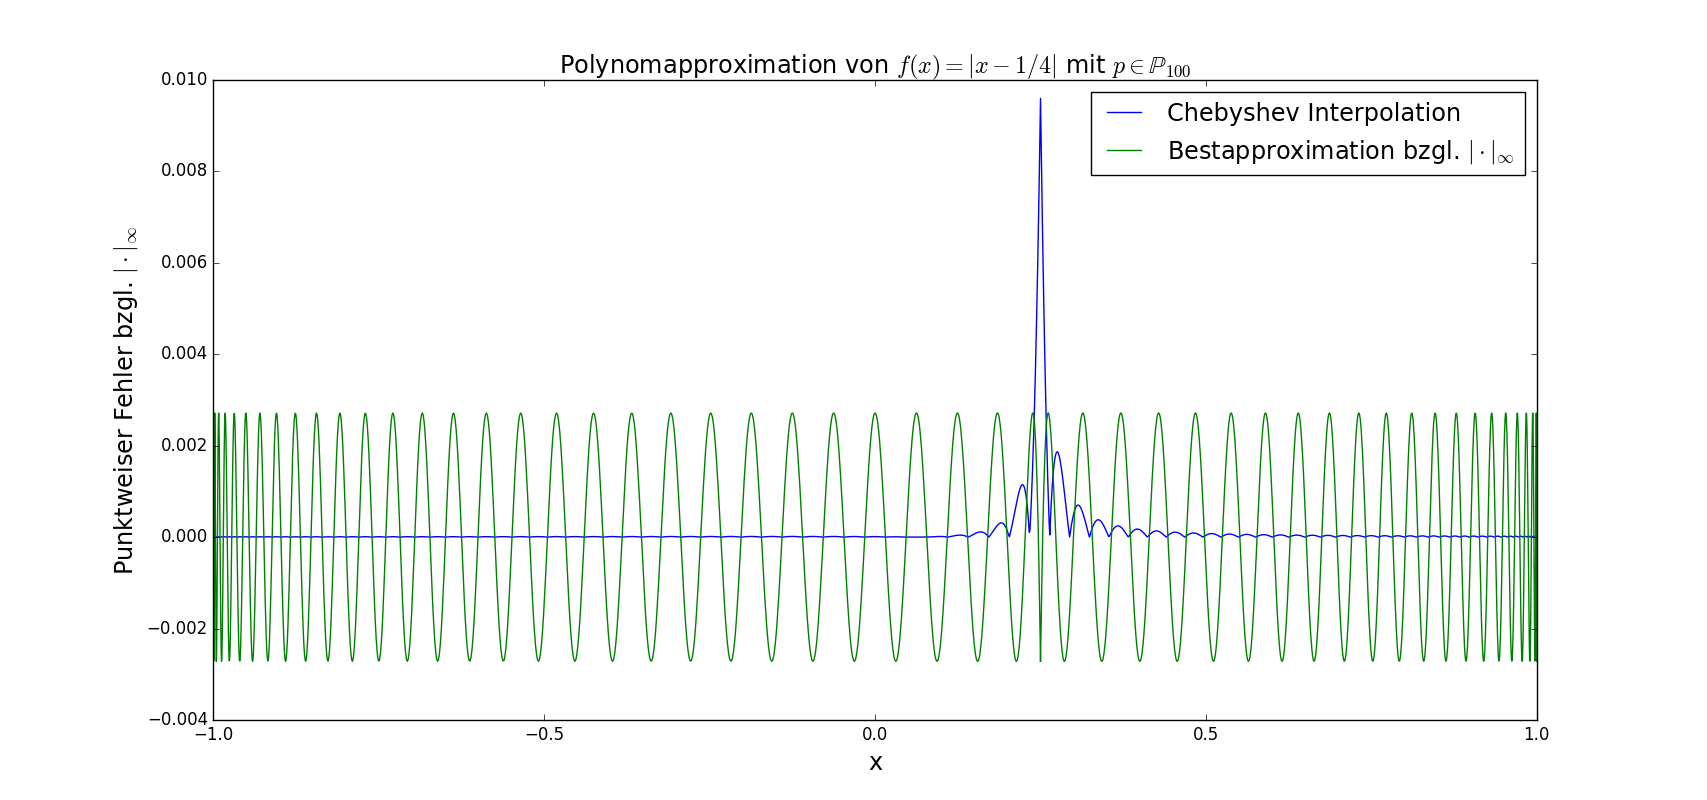
\includegraphics[width=\linewidth]{Figures/polynomial_approx_comparison.png}
 \caption{Visualisierung der Fehler verschiedener Approximationen, angelehnt an \autocite{Trefethen}. Hierbei wurde die Bestapproximation mithilfe des \emph{Remez} Algorithmus aus dem Chebfun Projekt (http://www.chebfun.org/) berechnet. Der Fehler der \chebyspace Approximation nimmt zu den Rändern hin stark ab.}
 \label{polyapproxcomp}
\end{figure}
\end{mathbsp}
Im Folgenden lösen wir uns von dem beschränkten Intervall $I$ und lassen auch $I=\R$ oder $I=[0,\infty)$ zu. Der Begriff der Bestapproximation lässt sich auch auf den Raum $L_w^2(I)$ erweitern. Dazu verwenden wir eine orthogonale Projektion auf eine orthogonale Polynombasis und erhalten eine einfache Darstellung des Bestapproximationsoperators.
\begin{maththeorem}
Ist $N\in\N_0$ und $\lbrace Q_k(x)\rbrace_{k=0}^N\subset \Poly_N$ ein Orthogonalsystem bezüglich des positiven Gewichtes $w(\cdot)$, also 
\[\langle Q_m(x),Q_n(x)\rangle_{L_w^2(I)}=\norm{Q_m}^2_{L_w^2(I)}\delta_{m,n},\quad, 0\le m,n\le N\]
so gilt für den Projektionsoperator $P_N\colon L_w^2(I)\to \Poly_N$ definiert durch 
\[P_Nf\coloneqq \sum_{k=0}^N\hat{f}_kQ_k(x),\quad \hat{f}_k\coloneqq \frac{1}{\norm{Q_k}_{L_w^2(I)}^2}\langle f,Q_k\rangle_{L_w^2(I)},\qquad f\in L^2_w(I),\]
die Bestapproximationsaussage
\[\norm{f-P_Nf}_{L_w^2(I)}=\inf\limits_{\psi\in\Poly_N}\norm{f-\psi}_{L_w^2(I)}\]
\end{maththeorem}
Dies entspricht der Fourier-Entwicklung im Hilbertraum. Entsprechend nennt man die Koeffizienten $\hat{f}_k$ die (verallgemeinerten) Fourier-Koeffizienten. Die Projektion ist eine Orthogonalprojektion in dem Sinne, dass der Fehler $f-P_Nf$ senkrecht zum Polynomraum $\Poly_N$ ist.\\
Wie schon bei der Bestapproximation bzgl. der Maximumsnorm erhält man auch für die verallgemeinerte Bestapproximation eine Konvergenzaussage. Für unbeschränktes $I$ sind die Beweise sehr aufwändig und beispielsweise in \autocite{CouHil53} zu finden. 
\begin{maththeorem}
Für jedes $f\in L_w^2(I)$ gilt
\[\lim\limits_{N\to\infty}\norm{f-P_Nf}_{L_w^2(I)}=0\]
\end{maththeorem}
Die Konvergenzordnung ist hierbei abhängig von der Regularität von $f$ und der Art der für die Projektion verwendeten Orthogonalpolynome. Man nennt diese Art der Konvergenz in der Literatur auch \emph{spektrale Konvergenz}, da die Konvergenzrate abhängig von der Glattheit der Funktion ist. Man muss also aufpassen eine hohe Approximationsordnung $N$ nicht mit einer hohen Approximationsgenauigkeit zu verwechseln.\\
Für das Beispiel der Legendre-Polynome, also mit konstanter Gewichtsfunktion $w$, zeigt Xiu in \autocite[Theorem 3.6]{dongbinxiu2010} folgendes Ergebnis.
\begin{maththeorem}
\label{spectralconvth}
Für jedes $f\in H_w^p[-1,1]\coloneqq \left\lbrace v\colon I\to\R | \frac{d^mv}{dx^m}\in L_w^2(I),0\le m\le p\right\rbrace$ mit $p\ge 0, w\equiv 1$ gibt es eine Konstante $C$ unabhängig von $N$, so dass
\[\norm{f-P_Nf}_{L_w^2[-1,1]}\le CN^{-p}\norm{f}_{H_w^p[-1,1]}\]
\end{maththeorem}
\begin{mathbsp}
Als Veranschaulichung von Satz \ref{spectralconvth} approximieren wir verschiedene Funktionen $f\colon [-1,1]\to\R$ durch die orthogonale Projektion $P_Nf$ für steigendes $N\in\N$. In Abbildung \ref{figurespectralconverg} sind dafür die Fehler der Approximationen dargestellt. Dabei sind die $f$ unterschiedlich glatt und man erkennt unterschiedliche Konvergenzordnungen. Insbesondere erahnt man für die analytische Funktion $f(x)=\sin(\pi x)$ exponentielle Konvergenz in $N$. Da der General-Purpose Integrator, der für die Berechnung der Fourierkoeffizienten verwendet wurde für zu hohe Polynomgrade versagt, bricht die Darstellung an der entsprechenden Stelle ab.
\begin{figure}[h]
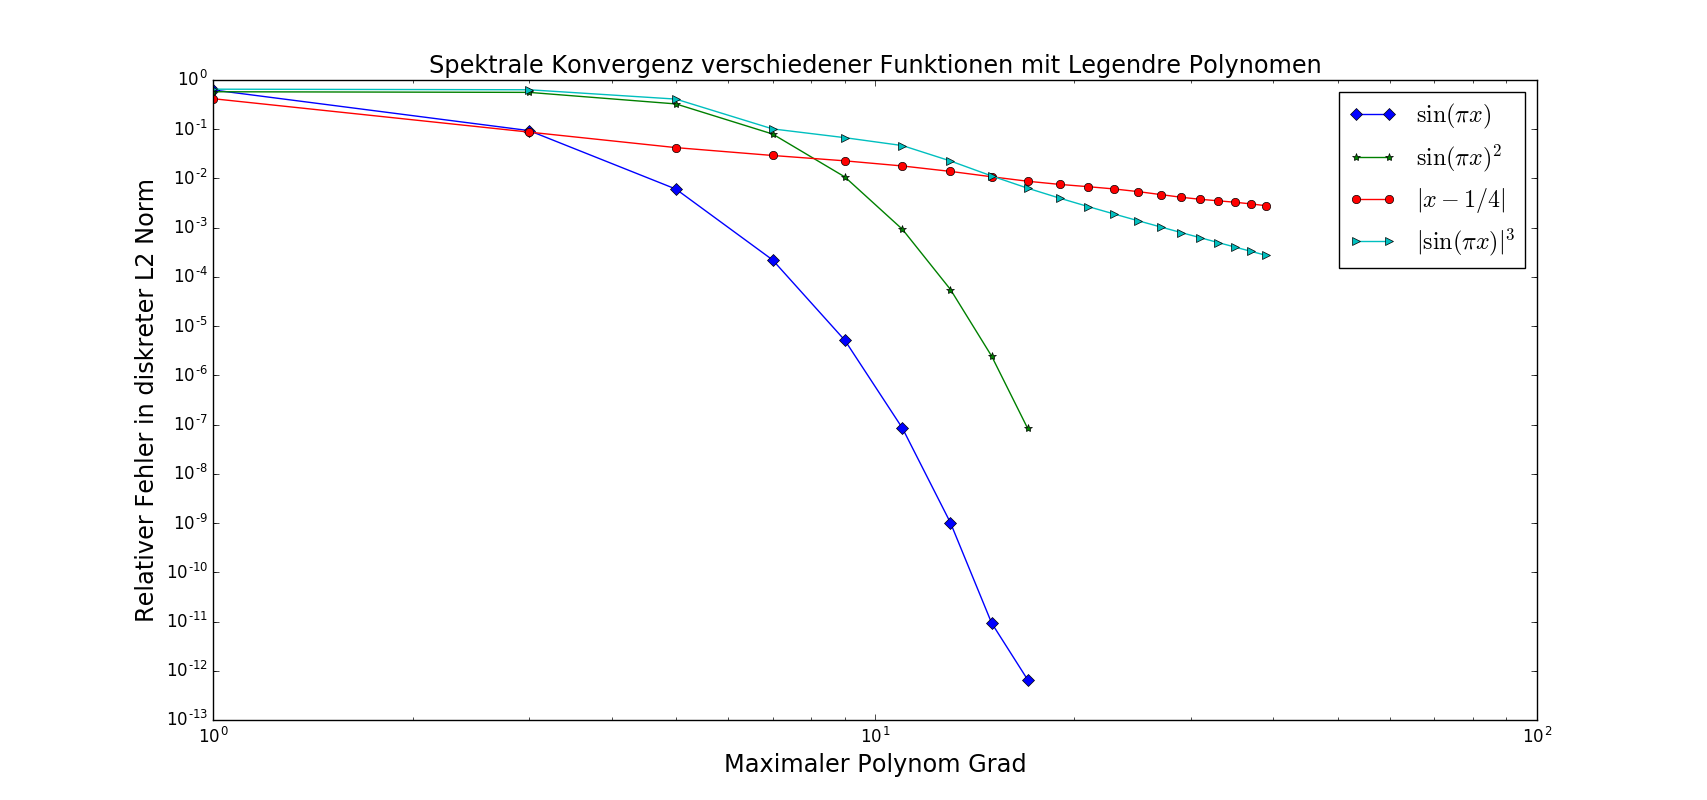
\includegraphics[width=\textwidth]{Figures/spectral_convergence_legendre.png}
\caption{Spektrale Konvergenz der Bestapproximation von Funktionen verschiedener Glattheit mithilfe von Legendre-Polynomen und Gewichtsfunktion $w\equiv \onehalf$ auf $[-1,1]$.}
\label{figurespectralconverg}
\end{figure}
\end{mathbsp}

\section{Approximation von Zufallsvariablen}
Anhand des Beispiels \ref{bsp:hermitechaos} des Hermite-Chaos haben wir bereits gesehen, dass für gewisse Orthonormalbasen von Polynomen $\lbrace H_i\rbrace$ und Zufallsvariablen $Y$ mit passenden stochastischen Verteilungen die Beziehung
\[\langle H_i(x),H_j(x)\rangle_{L_w^2(S)} =\E_Y \left[H_i(Y)H_j(Y)\right]=\delta_{ij}\]
erfüllt wird. Ein feiner Unterschied ist dabei, dass die Polynome einmal mit reellem Argument und einmal mit der Zufallsvariable $Y$ als Argument aufgefasst werden.
\begin{mathdef}[General Polynomial-Chaos Basis]
\label{def:gpc}
Sei $Y$ eine reelle Zufallsvariable mit Verteilungsfunktion $F_Y(y)=P(Y\le y)$ und endlichen Momenten
\[\E\left[|Y|^{2\ell}\right]=\int |y|^{2\ell}dF_Y(y)<\infty,\quad \ell\in \N_0\]
Existieren Polynome $\Phi_i\in\Poly_i$, insbesondere $\Phi_0\equiv const$, welche die Bedingung
\begin{equation}
\label{eqn:gpc_basicortho}
\E\left[\Phi_i(Y)\Phi_j(Y)\right]=\delta_{ij},\quad i,j\in\N_0
\end{equation}
erfüllen, so nennt man diese \emph{general Polynomial-Chaos Basis-Funktionen}.\\
Ist $Y$ stetig, so existiert eine Dichtefunktion $\rho>0$, so dass $dF_Y(y)=\rho(y)dy$ auf $I$. In diesem Fall lässt sich die Bedingung (\ref{eqn:gpc_basicortho}) schreiben als
\begin{equation}
\label{eqn:gpc_ortho}
\E\left[\Phi_i(Y)\Phi_j(Y)\right]=\int_I \Phi_i(y)\Phi_j(y)\rho(y)dy=\delta_{ij},\quad i,j\in\N_0
\end{equation}
\end{mathdef}
\begin{mathbem}
Betrachten wir die Orthogonalitätsbedingung (\ref{eqn:gpc_ortho}), so wird klar, dass diese direkt der Orthogonalität des Raumes $L_\rho^2(I)$ entspricht. Die Polynome erfüllen somit nach Satz \ref{threetermexist} eine Drei-Term-Rekursion und bilden eine Orthonormalbasis bezüglich $L_\rho^2(I)$.\\
Man beachte, dass die hier vorgenommene Normierung der Basis keine Beschränkung der Allgemeinheit darstellt. Gilt als Bedingung nur
\[\langle H_i,H_j\rangle_{L_w^2(S)} =\E_Y \left[H_i(Y)H_j(Y)\right]=\gamma_i\delta_{ij},\quad i,j\in\N_0,\gamma_i>0\]
so müssen die Polynome $H_i$ lediglich durch die Normalisierungskonstanten $\sqrt{\gamma_i}=\sqrt{\E\left[\Phi_i^2(Y)\right]}$ geteilt werden.\\
Ist $Y$ keine stetige sondern eine diskrete Zufallsvariable, so ändert sich die Notation und aus obigen Integralen würden Reihen, die Kernaussagen blieben aber dieselben. Wir werden jedoch im Folgenden stets stetige Zufallsvariablen verwenden.
\end{mathbem}
Eine Übersicht von einigen bekannten Verteilungen und Polynombasen ist in Tabelle \ref{table:chaos} gegeben. Details zu stetigen Verteilungen finden sich im Anhang \ref{AppendixA}.\\
\begin{table}
\centering
\begin{tabular}{c|ccc}
 & Verteilung von $Y$ & gPC-Basispolynome & Träger \\ 
\hline 
Stetig & Normal & Hermite & $(-\infty,\infty)$ \\ 
 & Gamma & Laguerre & $[0,\infty)$ \\ 
 & Beta & Jacobi & $[-1,1]$ \\
 & Gleich & Legendre & $[-1,1]$ \\  
\hline 
Diskret & Poisson & Charlier & $\lbrace 0,1,2,\dots\rbrace$ \\ 
 & Binomial & Krawtchouk & $\lbrace 0,1,\dots,E\rbrace$ \\ 
 & Negativ Binomial & Meixner & $\lbrace 0,1,2,\dots\rbrace$ \\  
 & Hypergeometrisch & Hahn & $\lbrace 0,1,\dots,E\rbrace$
\end{tabular}
\caption{gPC-Beziehung zwischen orthogonalen Polynombasen und stochastischen Verteilungen. $E\in\N_0$ ist dabei ein beliebiger Parameter für gewisse diskrete Verteilungen.}
\label{table:chaos}
\end{table}

Das Ziel ist nun, mithilfe einer gPC-Orthonormalbasis eine Funktion $f(Y)$ einer Zufallsvariablen $Y$ zu approximieren. Wir wollen nun einen Einblick dazu bekommen, was an dieser Stelle mit "`approximieren"' gemeint ist.
\begin{mathdef}[Starke gPC-Konvergenz]
Sei $f(Y)$ eine Funktion einer Zufallsvariablen $Y$ mit Dichte $\rho_Y$ und Träger $I_Y$. Eine general Polynomial-Chaos Approximation $f_M(Y)\in\Poly_M(Y)$ konvergiert in einem starken Sinne gegen $f(Y)$, wenn \[\norm{f(Y)-f_M(Y)}_{L_{\rho_Y}^2(I_Y)}\to 0\text{ für }{M\to\infty}\]
\end{mathdef}
Die starke gPC-Konvergenz entspricht also direkt der in Kapitel \ref{sec:poly_approx} vorgestellten spektralen Konvergenz, entsprechend ist die Konvergenzordnung abhängig von der Glattheit der Funktion $f$. Ohne Beweis folgt aus der starken gPC-Konvergenz auch die Konvergenz in Wahrscheinlichkeit und schlussendlich die Konvergenz in Verteilung.
\begin{mathbem}
Ist die Funktion $f$ oder ihre Abhängigkeit von der Zufallsvariablen $Y$ nicht konkret bekannt, sondern liegt diese beispielsweise nur als Verteilungsfunktion vor, so ist es dennoch möglich eine gPC-Approximation in einem schwachen Sinne zu erhalten. Für Details sei auf \autocite[Kapitel 5.1.2]{dongbinxiu2010} verwiesen.\\
Ein illustratives Beispiel ist in Abbildung \ref{fig:gpcweakconv} gegeben. Dort verwenden wir die Bestapproximation bezüglich $L_\rho^2(-\infty,\infty)$, wobei $\rho$ die Dichtefunktion der Normalverteilung ist, die Orthonormalbasis aus den Hermite-Polynomen $H_m$ besteht und $Y$ eine normalverteilte Zufallsvariable ist. Es ist
\[f_M(Y)=\sum_{m=0}^M\hat{f}_mH_m(Y), \quad \hat{f}_m=\E[f(Y)H_m(Y)]\]
die Bestapproximation an die Funktion $f(Y)$ in $\Poly_M(Y)$. Wir nehmen an, dass wir nur die Verteilung von $Z=f(Y)$ kennen und $Z\sim\text{Beta}(0.2,3.)$ in $[-1,1]$.\\
Dann tritt bei der Berechnung von $\E[ZH_m(Y)]$ eine Schwierigkeit auf: Es ist in dieser Form nicht möglich den Erwartungswert zu berechnen, da die Zufallsvariablen $Z$ und $H_m(Y)$ zu verschiedenen Wahrscheinlichkeitsräumen gehören. Hierzu ist es nun hilfreich, mithilfe der Inversionsmethode die beiden Verteilungen auf einen gemeinsamen Wahrscheinlichkeitsraum $\mathcal{U}(0,1)$ zu "`normieren"'. Dann gilt
\[\hat{f}_m=\E_U\left[F_Z^{-1}(U)H_m(F_Y^{-1}(U))\right]=\int_0^1F_Z^{-1}(u)H_m(F_Y^{-1}(u))du\]
und $f_M(Y)$ konvergiert in Verteilung gegen $f(Y)$ für $M\to\infty$.
\begin{figure}[!htb]
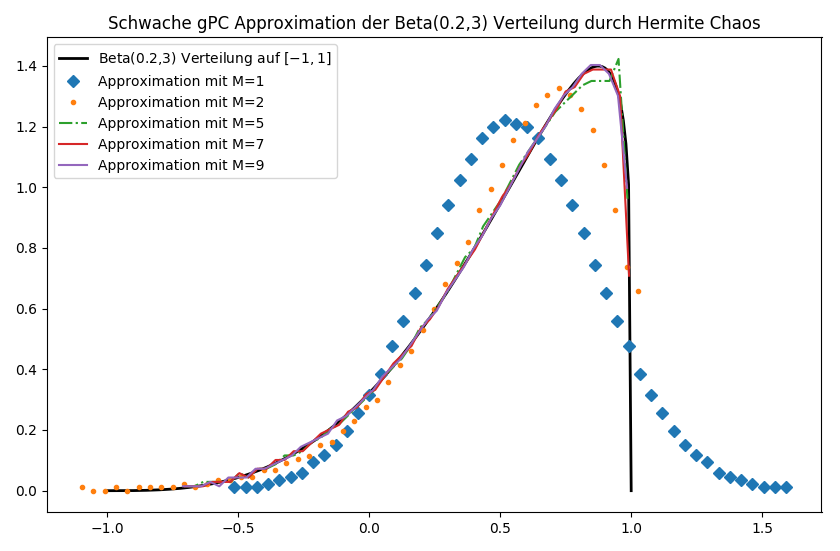
\includegraphics[width=\textwidth]{Figures/gpc_weak_convergence.png}
\caption{Schwache Konvergenz von Hermite gPC-Approximation zu einer $\text{Beta}(0.2,3.)$ verteilten Zufallsvariablen. Dargestellt sind Approximationen an die Dichtefunktionen, welche über Histogramme von 50 gleich großen Intervallen angenähert werden.}
\label{fig:gpcweakconv}
\end{figure}
\end{mathbem}

\section{Mehrdimensionale Zufallsräume}
Wie bereits diskutiert, sei der Zufallsraum durch einen Zufallsvektor $Y=(Y_1,\dots,Y_N)^T$ mit stochastisch unabhängigen Komponenten $Y_i$ mit bekannter Verteilung vollständig parametrisiert. Als mehrdimensionale Erweiterung von Definition \ref{def:gpc} führen wir an dieser Stelle das multivariate gPC-ein.
\begin{mathdef}[Multivariate gPC]
Sei $P\in\N_0$ der fest gewählte maximale Polynomgrad. Sei weiter $Y=(Y_1,\dots,Y_N)^T$ ein Zufallsvektor, dessen unabhängige Komponenten $Y_k$ eine gPC-Basis $\lbrace \Phi_i^{(k)}\in\Poly_P(Y_k)\mid i=0,\dots,P\rbrace$ besitzen. Ist $m=(m_1,\dots,m_N)\in\N_0^N$ ein Multi-Index mit $|m|=m_1+\dots+m_N$, so sind die $N$-variate gPC-Basis-Funktionen vom Grad $P$ definiert als 
\[\Phi_m(Y)=\Phi_{m_1}(Y_1)\cdot\ldots\cdot\Phi_{m_N}(Y_N),\quad 0\le |m|\le P\]
\end{mathdef}

\begin{mathbem}
Der von den multivariate gPC-Funktionen aufgespannte Raum $\Poly_P^N$ ist der Raum aller Polynome vom Grad höchstens $P$ in $N$ Variablen
\[\Poly_P^N(Y)\coloneqq \left\lbrace p\colon I_Y\to \R \mid p(Y)=\sum_{|m|\le P}c_m\Phi_m(Y)\right\rbrace\]
Die Dimension des Raumes ist $\dim\Poly_P^N=\binom{P+N}{P}=\frac{(P+N)!}{P!N!}$.
\end{mathbem}
\begin{proof}
Wir zeigen die zweite Aussage über die Dimension des Raumes. Die Beweisidee kann unter Verwendung von stochastischen Kombinationen direkt verwendet werden, um einen Algorithmus zur Generierung der Multi-Indices zu bekommen.\\
Da die Monome $x^m=x_1^{m_1}\dots x_N^{m_N}$ für verschiedene $m=(m_1,\dots,m_N)$ linear unabhängig und erzeugend sind, ist die Aussage äquivalent zur Aussage
\[\binom{P+N}{P}=\#\lbrace m\in\N_0^N \mid |m|\le P\rbrace\] 
Wir berechnen dazu $a_j=\#\lbrace m\in\N_0^N \mid |m|=j\rbrace$ für $j=0,\dots,P$. Dazu überlegen wir uns, dass $a_j=\#\lbrace \overline{m}\in\N^N \mid |\overline{m}|=j+N\rbrace$ wegen der Bijektion $m=(m_1,\dots,m_N)=(\overline{m}_1-1,\dots,\overline{m}_N-1)=\overline{m}-(1,\dots,1)$. Wir wollen nun herausfinden, wieviele Zerlegungen der Zahl $j+N=|\overline{m}|$ möglich sind und schreiben dazu symbolisch
\[\overline{m}=\underbrace{(1\_1\_1\_\dots 1\_1)}_{j+N\text{ Einsen getrennt von } j+N-1 \text{ Blanks}}\]
Um eine aller möglichen Darstellung zu bekommen, ersetzen wir $N-1$ Blanks durch ein Komma und die restlichen durch ein Plus, beispielsweise für $j=4,N=3$
\[(1+1+1,1,1+1+1+1+1)=(3,1,5)=\overline{m}\]
Dies sind exakt alle Möglichkeiten, $N$ positive Zahlen, deren Summe $j+N$ ist, zu erhalten, und es ist $a_j=\binom{j+N-1}{N-1}$.
Schlussendlich gilt für die Summe von verschobenen Binomialkoeffizienten 
\[\sum_{j=0}^Pa_j=\sum_{j=0}^P\binom{j+N-1}{N-1}\stackrel{\text{ind.}}{=}\binom{N+P}{N}=\binom{N+P}{P}\]
\end{proof}
Im Folgenden wird es sowohl für die theoretische Notation, als auch die konkrete Implementierung häufig praktischer sein, die Multi-Indices $m\in\N_0^M$ durchzunummerieren und äquivalent zum eindimensionalen Fall zu benutzen. Dies ist gerechtfertigt, da sich die zugehörigen multivariaten Polynome ähnlich wie die eindimensionalen Polynome verhalten. Zum Beispiel gilt aufgrund des gewählten Tensorproduktansatzes und der stochastischen Unabhängigkeit der Komponenten von $Y$ das mehrdimensionale Pendant zur Orthogonalitätsbedingung (\ref{eqn:gpc_ortho}) für $i,j\in\N_0^N$
\begin{equation}
\label{eqn:gpc_ortho_mv}
\begin{split}
&\E\left[\Phi_i(Y)\Phi_j(Y)\right]=\int_{I_Y} \Phi_i(y)\Phi_j(y)\rho(y)dy\\
&=\int_{I_{Y_1}}\dots\int_{I_{Y_N}}\Phi_{i_1}(y_1)\dots\Phi_{i_N}(y_N)\Phi_{j_1}(y_1)\dots\Phi_{j_N}(y_N)\\
&\qquad\quad\cdot\rho_{Y_1}(y_1)\dots\rho_{Y_N}(y_N)dy_N\dots dy_1\\
&=\int_{I_{Y_1}}\Phi_{i_1}(y_1)\Phi_{j_1}(y_1)\rho_{Y_1}(y_1)dy_1\dots\int_{I_{Y_N}}\Phi_{i_N}(y_N)\Phi_{j_N}(y_N)\rho_{Y_N}(y_N)dy_N\\
&=\delta_{i_1j_1}\dots \delta_{i_Nj_N}=\delta_{ij}
\end{split}
\end{equation}
In diesem Sinne gilt dann für die mehrdimensionale Bestapproximation die selbe Darstellung $f_M(Y)=\sum_{m=0}^M\hat{f}_mH_m(Y)$, wobei $M+1=\binom{N+P}{P}$ die Anzahl an Basispolynomen ist und $P$ die Schranke der Multi-Indices $|m|\le P$.\\
Für eine eindeutige Nummerierung der Indices benötigen wir eine Sortierung. Wir einigen uns als Sortierung der Indices auf die Termordnung (engl. \emph{graded lexicographic order}), die für $i,j\in\N_0^N$ gegeben ist durch 
\[i>j \equivalent |i|\ge |j| \text{ und der erste nicht-negative Eintrag von } i-j \text { ist positiv}\]
Für $N=3$ sind für $|m|=0,\dots,2$ die ersten Multi-Indices gegeben durch
\begin{align*}
&(0,0,0)\\
&(1,0,0)<(0,1,0)<(0,0,1)\\
&(2,0,0)<(1,1,0)<(1,0,1)<(0,2,0)<(0,1,1)<(0,0,2)\\
\end{align*}
\begin{mathbem}
Die Wahl der beschränkten Summe $|m|\le P$ für $m\in\N_0^N$ ist eine Einschränkung an den Polynomraum, den wir für die Approximation verwenden wollen. Häufig ist für theoretische Überlegungen der volle Tensorproduktraum mit $m_i\le P$ für alle $i=1,\dots,N$ der Raum der Wahl, da sich dann Ergebnisse aus dem eindimensionalen direkter auf den mehrdimensionalen Fall übertragen lassen. Die Dimension des vollen Tensorproduktraumes beträgt jedoch $(P+1)^N$, was bereits für kleine Dimensionen $N$ eine große Anzahl an Basispolynomen bedeuten würde und folglich einen hohen Rechenzeitaufwand (vgl. Tabelle \ref{table:poly_space_dim}).
\begin{table}
\centering
\begin{tabular}{c|cc}
$P$ & $\binom{P+N}{P}$ & $(P+1)^N$\\
\hline
1  &  5  &  16 \\
2  &  15  &  81 \\
3  &  35  &  256 \\
4  &  70  &  625 \\
5  &  126  &  1,296 \\
10  &  1,001  &  14,641 \\
100  &  4,598,126  &  104,060,401 
\end{tabular}
\caption{Vergleich der Dimensionen der verschiedenen Approximationsräume für $N=4$ und unterschiedliche $P$.}
\label{table:poly_space_dim}
\end{table}
\end{mathbem}
Als weitere Motivation für unsere Wahl des Polynomraums geben wir ein Beispiel an, anhand dessen wir das Verhalten der Koeffizienten der Bestapproximation beobachten können.
\begin{mathbsp}
\label{bsp:bestapproxcoeffs2d}
Sei $N=2, Y=(Y_1,Y_2)^T$ mit $Y_1\sim \mathcal{U}(-1,1), Y_2\sim\mathcal{N}(0,1)$ und die zu approximierende Funktion $f(y)=f(y_1,y_2)=(2+\sin(y_1\cdot y_2))^{-2}$.\\
Wir betrachten die Koeffizienten $\hat{f}_m$ der Bestapproximation \[f_M(y)=\sum_{m_1=0}^P\sum_{m_2=0}^P\hat{f}_m\Phi_m(y)\] im vollständigen Tensorproduktraum. Dabei wählen wir die zu den Verteilungen passenden Polynome $\Phi_m(y)=L_{m_1}(y_1)H_{m_2}(y_2)$, wobei $L_{m_1}$ die normierten Legendre-Polynome und $H_{m_2}$ die normierten Hermite-Polynome sind. Für die Koeffizienten gilt
\[\hat{f}_m=\int_{-1}^1\int_{-\infty}^\infty f(y_1,y_2)\cdot \onehalf \cdot \frac{1}{\sqrt{2\pi}}e^{-\frac{y_2^2}{2}}\cdot L_{m_1}(y_1)\cdot H_{m_2}(y_2)dy_2dy_1\]
In Abbildung \ref{fig:bestapproxcoeffs2d} ist der Betrag der Koeffizienten $|\hat{f}_m|$ in einem Gitter eingezeichnet. Die schwarze Linie symbolisiert die Grenze derjenigen Indices, die $|m|\le 22$ erfüllen. Wir sehen, dass die Koeffizienten im oberen rechten Eck, die zu Polynomen wie $L_{17}H_{17}$ gehören, betragsmäßig sehr klein in der Größenordnung $10^{-6}$ sind. Die volle Tensorapproximation bietet in diesem Fall also nur geringe Vorteile gegenüber der Approximation mit $|m|\le 22$. Der Verzicht auf diejenigen Polynome mit hohem gemischten Grad $|m|$ erspart also viel Aufwand und bietet dennoch eine gute Approximation, da das Abklingverhalten der Koeffizienten häufig durch die eingezeichnete Diagonale dominiert wird.
\begin{figure}[!htb]
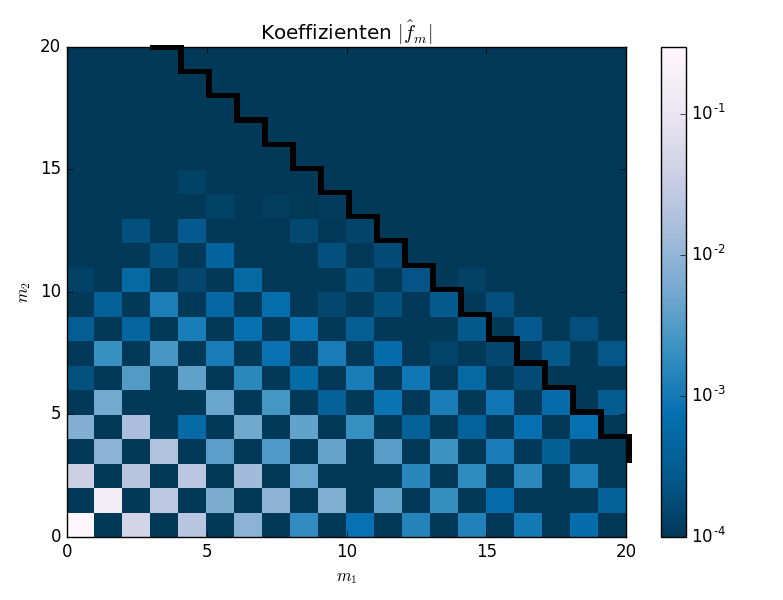
\includegraphics[width=\textwidth]{Figures/best_approx_coeffs_2d_example2log.png}
\caption{Koeffizienten $|\hat{f}_m|$ der Bestapproximation für $m_1,m_2=0,\dots,15$ der Funktion aus Beispiel \ref{bsp:bestapproxcoeffs2d}. Koeffizienten links unterhalb der schwarzen Linie erfüllen dabei $|m|\le 22$.}
\label{fig:bestapproxcoeffs2d}
\end{figure}
\end{mathbsp}

\section{Extraktion von Statistiken}
Gegeben sei die multivariate gPC-Approximation mit Summenschranke $P$ zu einer Funktion $f(Y)$ und einem Zufallsvektor $Y$ der Dimension $N$, also
\[f(Y)\approx f_M(Y)=\sum_{|m|\le P}\hat{f}_m\Phi_m(Y)\in\Poly_P^N,\quad m\in\N_0^N\]
Unter Ausnutzung der Orthogonalitätsbedingung (\ref{eqn:gpc_ortho_mv}) der Polynombasen lassen sich gewisse Statistiken der gPC-Approximation auf sehr einfache Art und Weise berechnen. Schlussendlich ist dies eine der größten Motivationen dafür, die Orthogonalbasis passend zur gegebenen Verteilung zu wählen.\\
Es ist $\gamma_{(0,\dots,0)}=1$, da für das nicht normalisierte Polynom $\Psi_0\equiv 1$ und eine Wahrscheinlichkeitsverteilung $F_Y$ gilt $\gamma_0=\E[\Psi_0^2(Y)]=\int 1\cdot 1dF_Y(y)=1$. Folglich gilt $\Phi_{(0,\dots,0)}(Y)= \frac{\Psi_0(Y)}{\sqrt{\gamma_0}}\equiv 1$ und für den Erwartungswert $\mu_f$
\begin{equation}
\label{eqn:gpc_approx_exp}
\begin{split}
\mu_f=\E[f(Y)]\approx \E[f_N(Y)]&=\int\left(\sum_{|m|\le P}\hat{f}_m\Phi_m(Y)\right)dF_Y(y)\\
&=\sum_{|m|\le P}\hat{f}_m\int\Phi_m(Y)dF_Y(y)\\
&=\sum_{|m|\le P}\hat{f}_m\E[\underbrace{\Phi_{(0,\dots,0)}(Y)}_{\equiv 1} \Phi_m(Y)]\\
&=\sum_{|m|\le P}\hat{f}_m\delta_{(0,\dots,0),m}=\hat{f}_{(0,\dots,0)}
\end{split}
\end{equation}
Die Varianz lässt sich dann berechnen als
\begin{align*}
\sigma^2_f=\text{var}(f(Y))&=\E[f^2(Y)]-\E[f(Y)]^2\\
&\approx \sum_{|m|\le P}\sum_{|n|\le P}\hat{f}_m\hat{f}_n\underbrace{\E[\Phi_m(Y)\Phi_n(Y)]}_{=\delta_{mn}}-\hat{f}_{(0,\dots,0)}^2\\
&=\sum_{0<|m|\le P}\hat{f}_m^2
\end{align*}
Die Standardabweichung ist folglich gegeben durch
\[\sigma_f=\sqrt{\text{var}(f(Y))}\approx\sqrt{\sum_{0<|m|\le P}\hat{f}_m^2}\]
Ist man an einer Approximation der Dichtefunktion von $f(Y)$ interessiert, so lässt sich diese mittels eines Histogramms und Samplings der Funktion $f_N(Y)=\sum_{|m|\le P}\hat{f}_m\Phi_m(Y)$ näherungsweise darstellen.\\[0.2cm]
Für höhere Momente gilt
\begin{align*}
\E[f^\ell(Y)]\approx \sum_{|m^{(1)}|,\dots,|m^{(\ell)}|\le P} \hat{f}_{m^{(1)}}\dots\hat{f}_{m^{(\ell)}}\underbrace{\E[\Phi_{m^{(1)}}(Y)\dots\Phi_{m^{(\ell)}}(Y)]}_{=\mathcal{T}_{m^{(1)},\dots m^{(\ell)}}}
\end{align*}
Diese Berechnung benötigt für $\ell>2$ eine einmalige Berechnung des Tensors $\mathcal{T}$. Dieser ist unabhängig von der betrachten Funktion $f$ und kann somit wieder verwendet werden.
\begin{mathbsp}
Für $N=1$ und $\ell=3$ ist der Momententensor $\mathcal{T}$ für $Y\sim \mathcal{N}(0,1)$ und zugehöriger orthonormaler Polynombasis $H_m$ der Hermite-Polynome für $P=2$ gegeben durch
\[\mathcal{T}=
\begin{tikzpicture}[every node/.style={anchor=north east,fill=white,minimum width=0.7cm,minimum height=7mm}]
\matrix (mA) [draw,matrix of math nodes]
{
0 & 0 & 1 \\
0 & \sqrt{2} & 0 \\
1 & 0 & 2\sqrt{2} \\
};

\matrix (mB) [draw,matrix of math nodes] at ($(mA.south west)+(0.2,1.5)$)
{
0 & 1 & 0 \\
1 & 0 & \sqrt{2} \\
0 & \sqrt{2} & 0 \\
};

\matrix (mC) [draw,matrix of math nodes] at ($(mB.south west)+(0.2,1.5)$)
{
 1 & 0 & 0 \\
 0 & 1 & 0 \\
 0 & 0 & 1 \\
};

\draw[dashed](mA.north east)--(mC.north east);
\draw[dashed](mA.north west)--(mC.north west);
\draw[dashed](mA.south east)--(mC.south east);
\end{tikzpicture}
\]
\end{mathbsp}